\documentclass{article}
\usepackage{amsmath}
\usepackage{unixode}
% \usepackage{amsthm,amssymb}
\usepackage{graphicx}
% \usepackage{longtable}
\usepackage{booktabs}
\usepackage[top=1cm, left=2cm,right=2cm,bottom=1cm]{geometry}%

\begin{document}

\noindent Consider the following Hidden Markov Model.

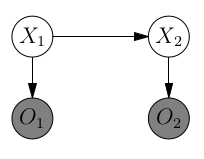
\includegraphics[scale=0.5]{hmm.png}
% \begin{longtable}[]{@{}ll@{}}
%   {@{}ll@{}}

\begin{tabular}{c|c}
X₁ & Pr(X₁)\tabularnewline
\midrule
% \endhead
0 & 0.3\tabularnewline
1 & 0.7\tabularnewline
  \end{tabular}
% \end{longtable}
  \hfill
  \begin{tabular}{c|c|c}
% \begin{longtable}[]{@{}lll@{}}
Xₜ & Xₜ₊₁ & Pr(Xₜ₊₁ ∣ Xₜ )\tabularnewline
\midrule
% \endhead
0 & 0 & 0.4\tabularnewline
0 & 1 & 0.6\tabularnewline
        \midrule
1 & 0 & 0.8\tabularnewline
1 & 1 & 0.2\tabularnewline
  \end{tabular}
% \end{longtable}
% \begin{longtable}[]{@{}lll@{}}
  \hfill
  \begin{tabular}{c|c|c}
Xₜ & Oₜ & Pr(Oₜ ∣ Xₜ)\tabularnewline
\midrule
% \endhead
0 & A & 0.9\tabularnewline
0 & B & 0.1\tabularnewline
        \midrule
1 & A & 0.5\tabularnewline
1 & B & 0.5\tabularnewline
  \end{tabular}
  \vskip5mm
\noindent Use the Forward algorithm to compute the probability distribution
Pr(X₂, O₁ = A, O₂ = B). Show your work. You do not need to evaluate arithmetic expressions involving only
numbers.

\vskip5mm
\noindent \textbf{Solution}.
We must compute Pr(X₂, O₁ = A, O₂ = B) for each value of X₂. That is, we
compute the two probabilities Pr(X₂ = 0, O₁ = A, O₂ = B) and Pr(X₂ = 1,
O₁ = A, O₂ = B). We do this by first computing Pr(X₂ = 0, x₁, O₁ = A, O₂
= B) for each x₁ ∈ \{0, 1\} (the possible values for the random variable
X₁), and then we sum over x₁ to get the marginal probability Pr(X₂ = 0,
O₁ = A, O₂ = B).
\[
\rm{Pr}(X₂, O₁ = A, O₂ = B) = ∑_{x₁} Pr(X₂, x₁, O₁ = A, O₂ = B).
\]
Recall, by the definition of conditional probability (or the chain
rule), we have
\begin{align*}
  \rm Pr(X₂, x₁, O₁ = A, O₂ = B) &= \rm Pr(x₁) Pr(X₂, O₁ = A, O₂ = B ∣ x₁)\\
                             &= \rm Pr(x₁) P(O₁ = A∣ x₁)Pr(X₂, O₂ = B ∣ x₁, O₁ = A)\\
                             &= \rm Pr(x₁) P(O₁ = A∣ x₁)Pr(X₂ ∣ x₁, O₁ = A)Pr(O₂ = B∣ X₂, x₁, O₁ = A)
\end{align*} Now we use the structure of the Bayes net to infer some
conditional independences and simplify the above express. Specifically,
O₂ is independent of O₁ given X₂ and O₂ is independent of X₁ given X₂.
% , so Pr(O₂ = B ∣ X₂, x₁,O₁ = A) = Pr(O₂ = B ∣ X₂).
Also, X₂ is independent of O₁ given X₁.
% , so Pr(X₂∣ x₁, O₁= A) = Pr(X₂∣ x₁).
Therefore, Pr(X₂, x₁, O₁ = A, O₂ = B) = Pr(x₁) Pr(O₁ = A ∣ x₁)Pr(X₂∣ x₁) Pr(O₂ = B ∣ X₂).
We now use the data in the tables above to compute
\begin{align*}
  \rm Pr(X₂ = 0, X₁ = 0, O₁ = A, O₂ = B) &= \rm Pr(X₁ = 0) Pr(O₁ = A∣ X₁ = 0) Pr(X₂ = 0∣ X₁ = 0) Pr(O₂ = B ∣ X₂ = 0)\\
                                     &= 0.3 · 0.9 · 0.4 · 0.1, \text{ and }
\end{align*}
\begin{align*}
  \rm Pr(X₂ = 0, X₁ = 1, O₁ = A, O₂ = B) &= \rm Pr(X₁ = 1) Pr(O₁ = A∣ X₁ = 1) Pr(X₂ = 0∣ X₁ = 1) Pr(O₂ = B ∣ X₂ = 0)\\
                                     &= 0.7 · 0.5 · 0.8 · 0.1
\end{align*} Therefore, Pr(X₂ = 0, O₁ = A, O₂ = B) = 0.3 · 0.9 · 0.4
· 0.1 + 0.7 · 0.5 · 0.8 · 0.1 = 0.1 (0.3 · 0.9 · 0.4 + 0.7 · 0.5 · 0.8)
= 0.1 (0.108 + 0.280) = 0.0388, Similarly,
\begin{align*}
  \rm Pr(X₂ = 1, X₁ = 0, O₁ = A, O₂ = B) &= \rm Pr(X₁ = 0) Pr(O₁ = A∣ X₁ = 0) Pr(X₂ = 1∣ X₁ = 0) Pr(O₂ = B ∣ X₂ = 1)\\
                                     &= 0.3 · 0.9 · 0.6 · 0.5,  \text{ and }
\end{align*}
\begin{align*}
  \rm Pr(X₂ = 1, X₁ = 1, O₁ = A, O₂ = B) &= \rm Pr(X₁ = 1) Pr(O₁ = A∣ X₁ = 1) Pr(X₂ = 1∣ X₁ = 1) Pr(O₂ = B ∣ X₂ = 1)\\
                                     &= 0.7 · 0.5 · 0.2 · 0.5
\end{align*} Therefore, Pr(X₂ = 1, O₁ = A, O₂ = B) = 0.3 · 0.9 · 0.6
· 0.5 + 0.7 · 0.5 · 0.2 · 0.5 = 0.5 (0.3 · 0.9 · 0.6 + 0.7 · 0.5 · 0.2)
= 0.5 (0.162 + 0.07) = 0.1160, So the distribution Pr(X₂, O₁ = A, O₂ = B) is given by the following table:
\begin{center}
\begin{tabular}{l|c}
% \begin{longtable}[]{@{}ll@{}}
X₂ & Pr(X₂, O₁ = A, O₂ = B)\tabularnewline
\midrule
0 & 0.0388\tabularnewline
1 & 0.1160\tabularnewline
\end{tabular}
\end{center}
% \end{longtable}
\end{document}
